\subsection{Subsequence Matching in Time-Series CPU statistics}
\label{sec:kookjin}

\subsubsection{Overview:}
In this section, we describe 1) how the collected raw data are processed to be useful in building up datasets and 2) how the processed data are stored in the datasets.

To efficiently match a subsequence, a query sequence, to the collected video sequence in the dataset, we converted the time series datasets (i.e. the video sequence and the query sequence) into datasets in spatial space. To build-up the datasets largely consists of two jobs: pre-processing raw data sequences and storing the processed sequences into a data structure.

\subsubsection{Pre-processing raw data sequences:}
For the same movie title, we collected cpu statistics for five times under the same environment. To remove the noise in the raw data, we used the Savitzky-Golay smoothing filter which is commonly used to filter out noise in time series data \cite{SGfilter}. The SG filter averages n adjacent points to flatten noise while preserving features of the distribution. In the experiment, we set the window length as 300. After smoothing, five cpu statistic streams were averaged because each statistic has little different amplitudes. Before averaging, streams needed to be aligned and trimmed appropriately because the data collection was manually done by hands. We set the first stream of each movie as a reference to the other 4 streams, and performed cross-correlation to obtain a time-lag which gives a point where streams are most similar. Once the alignment was done, the amplitude of five streams are averaged, and the sequence with the averaged amplitude was stored in the datasets and was used as the reference sequence to a query sequence.

To convert the pre-processed sequences into data trails in the spatial domain, Discrete Fourier Transform (DFT) was applied to the pre-processed sequences. More specifically, a  DFT window of a specified length is used so that DFT could be applied to each subsequence within a video sequence from the starting index to the end index of the video sequence. At every DFT application to each subsequence, the first two Fourier coefficients were extracted, which made the time series data sequence to be 2-dimensional spatial data while preserving more than 80-percent of energy of the original sequence.

\begin{figure}[!t]
	\centering
	\subfigure[Raw sequence] {
		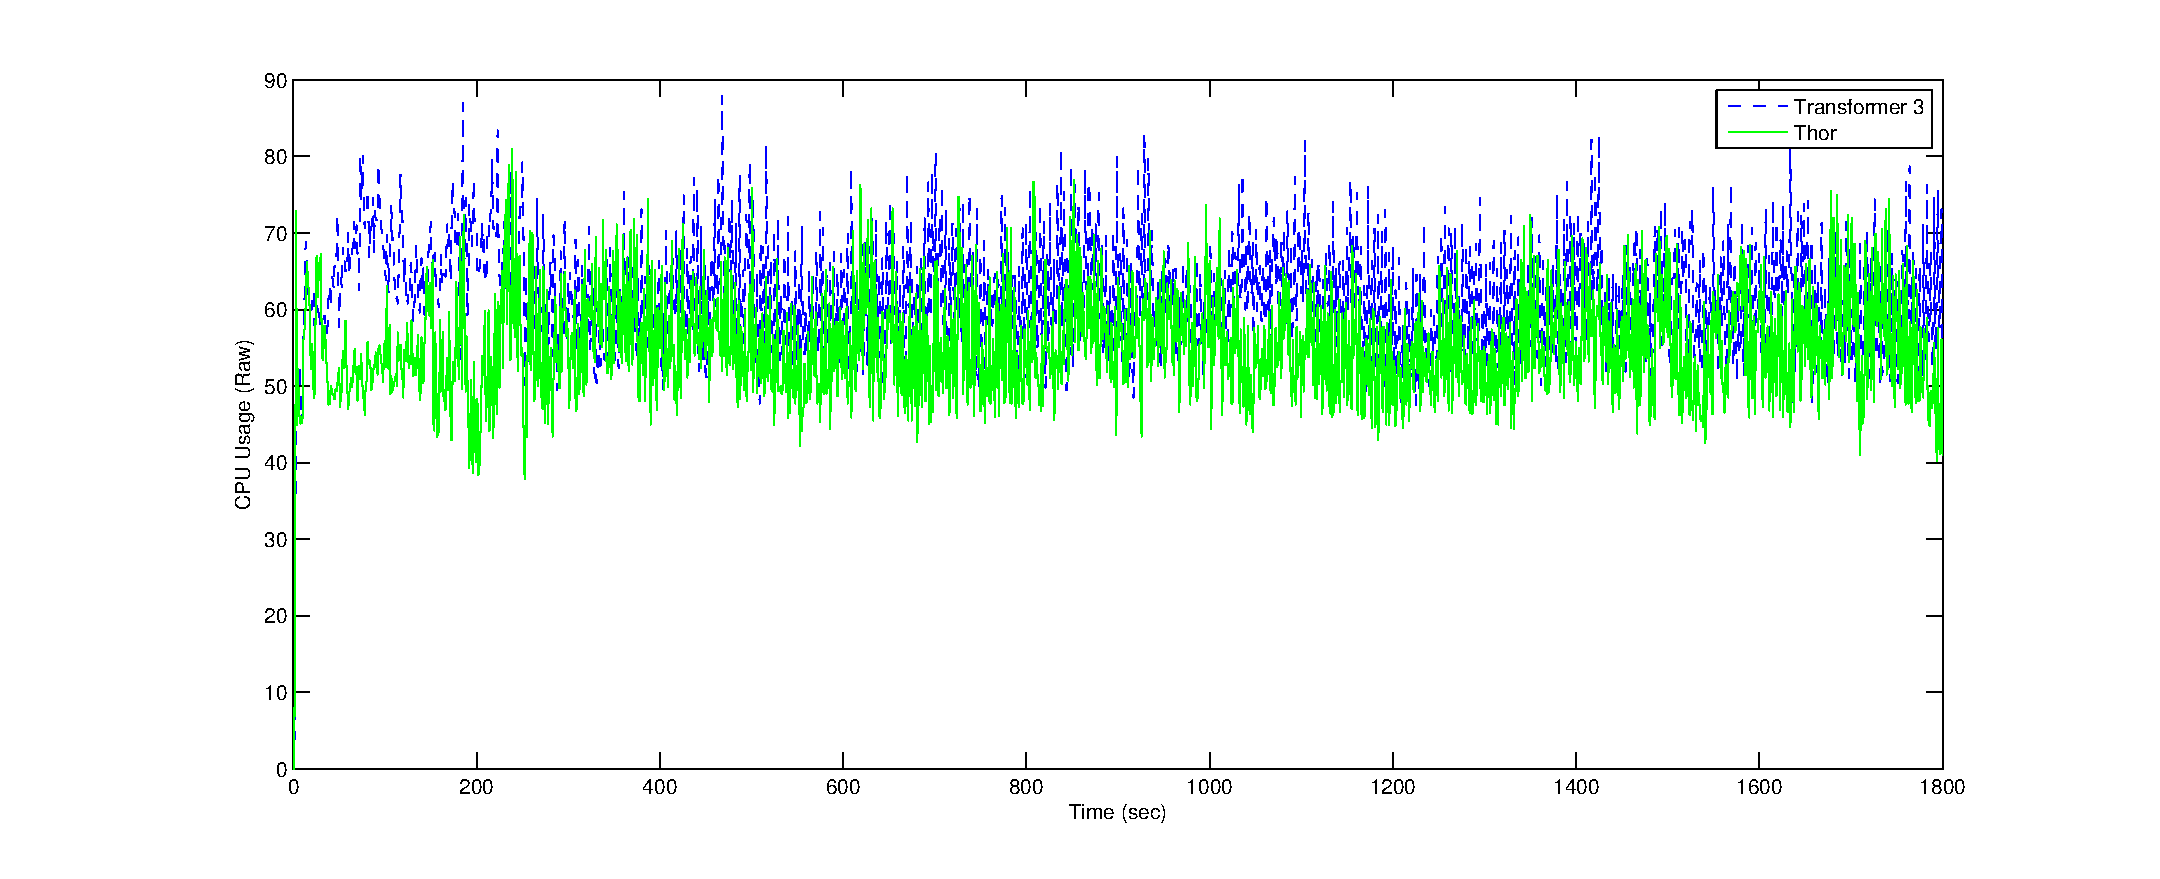
\includegraphics[scale=0.225]{Figures/RAW_TF_Thor}
	}
	\subfigure[Smoothed sequence] {
		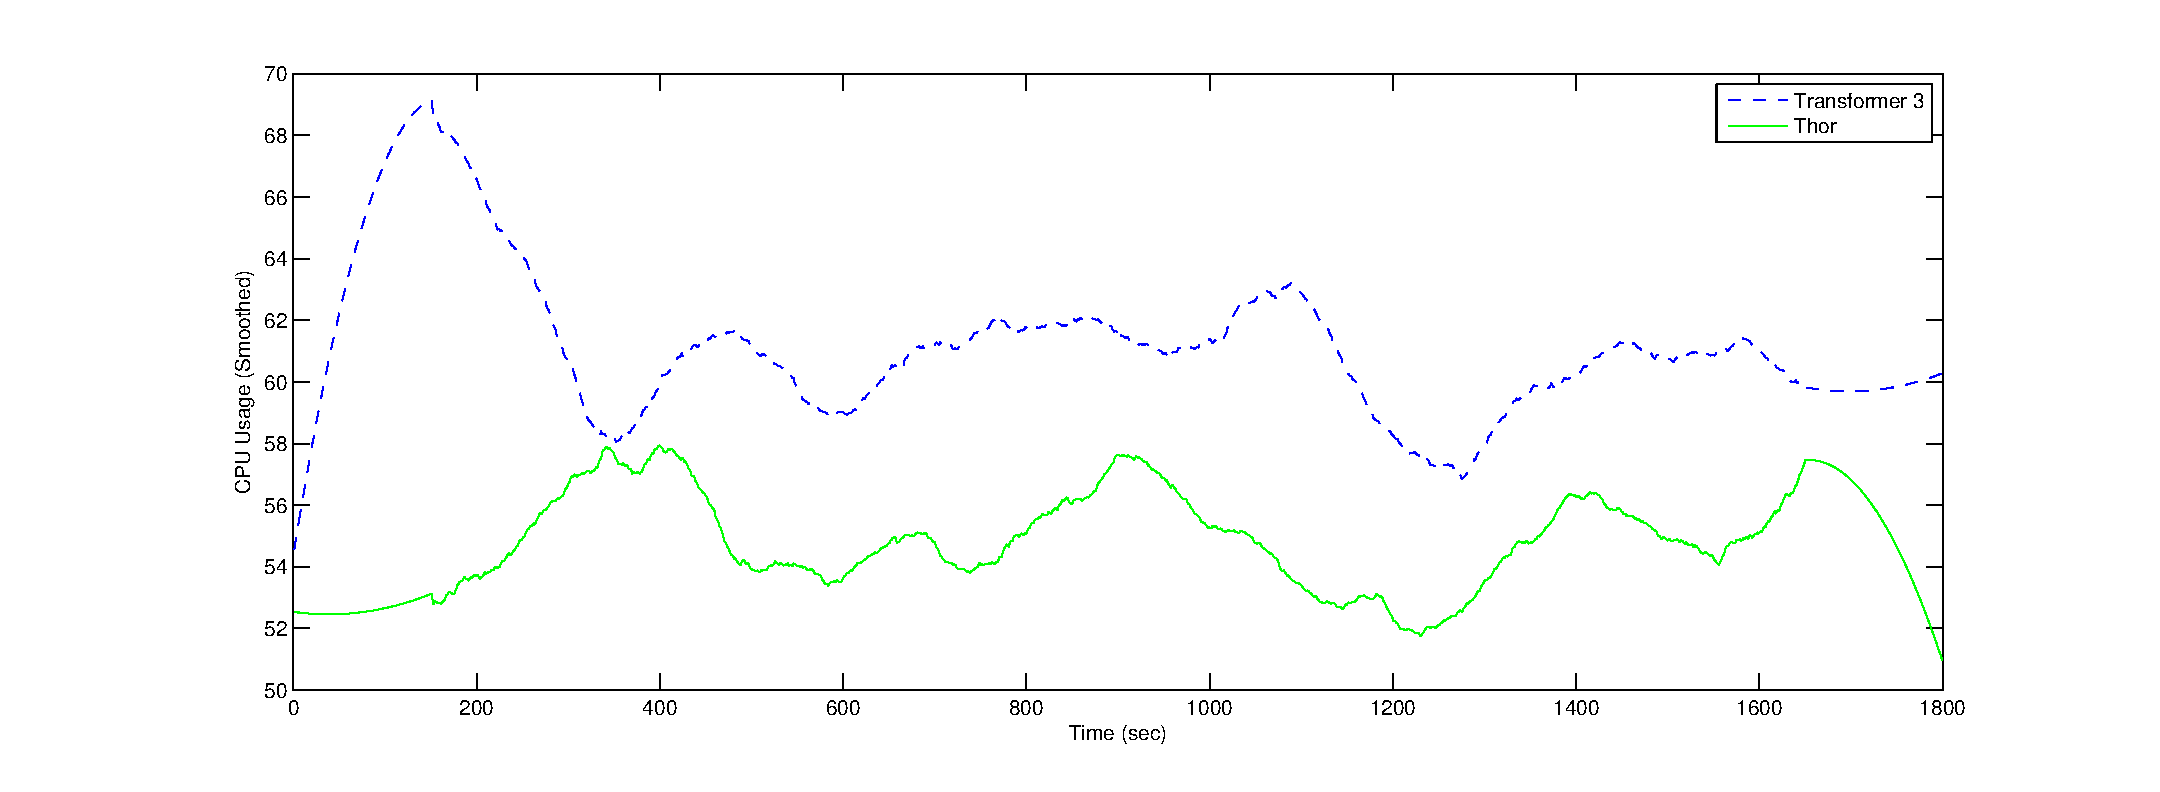
\includegraphics[scale=0.225]{Figures/SMTH_TF_Thor}
	}
	\subfigure[Aligned sequences and averaged sequence] {
		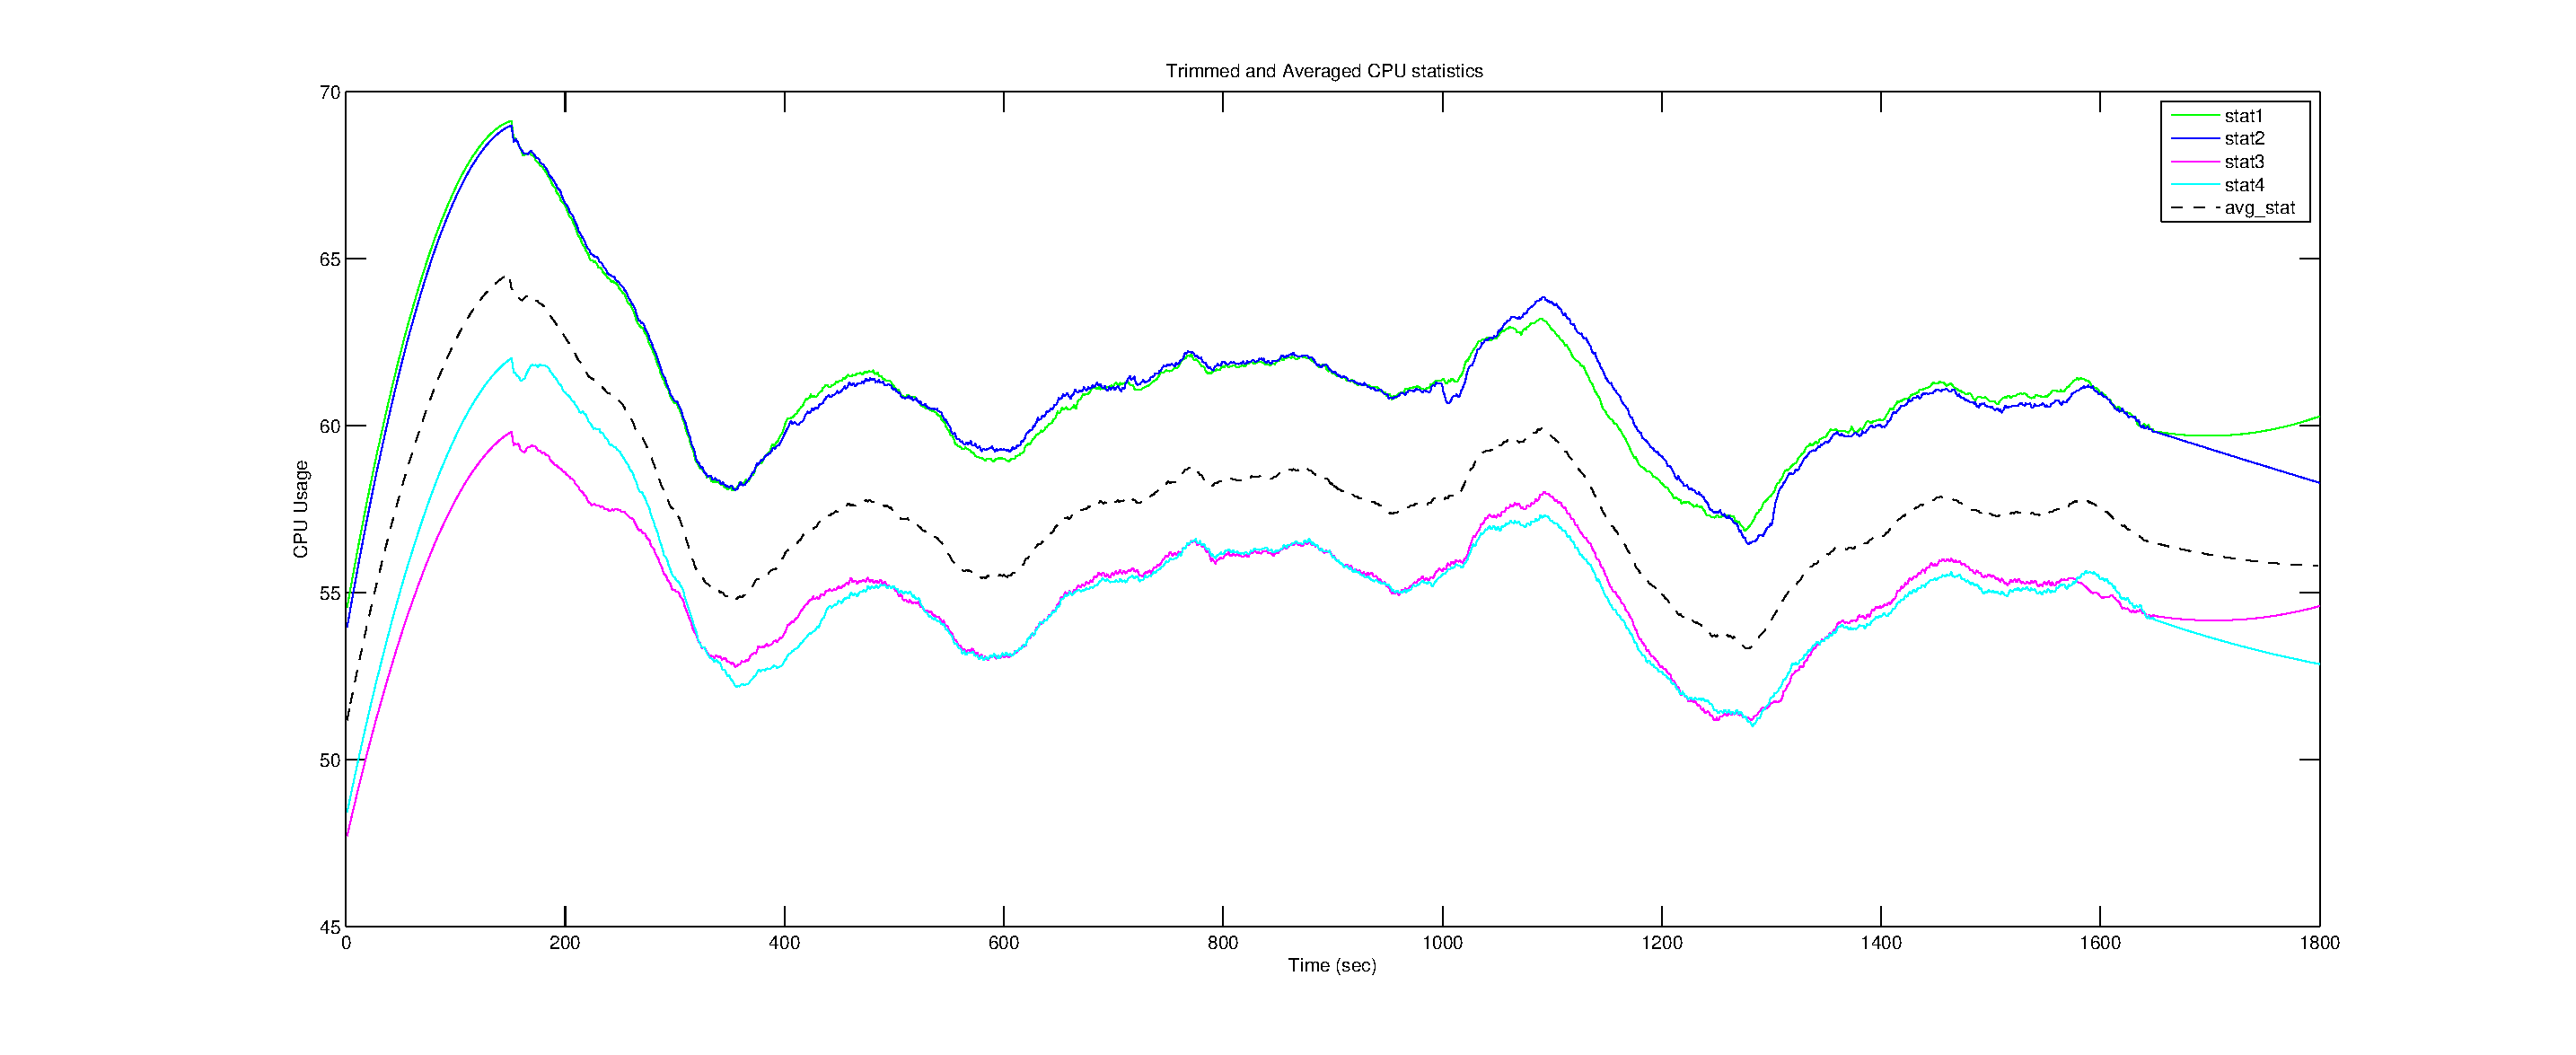
\includegraphics[scale=0.225]{Figures/Trim_Avg_TF}
	}
	\subfigure[A FFT filtered sequence of two movies] {
		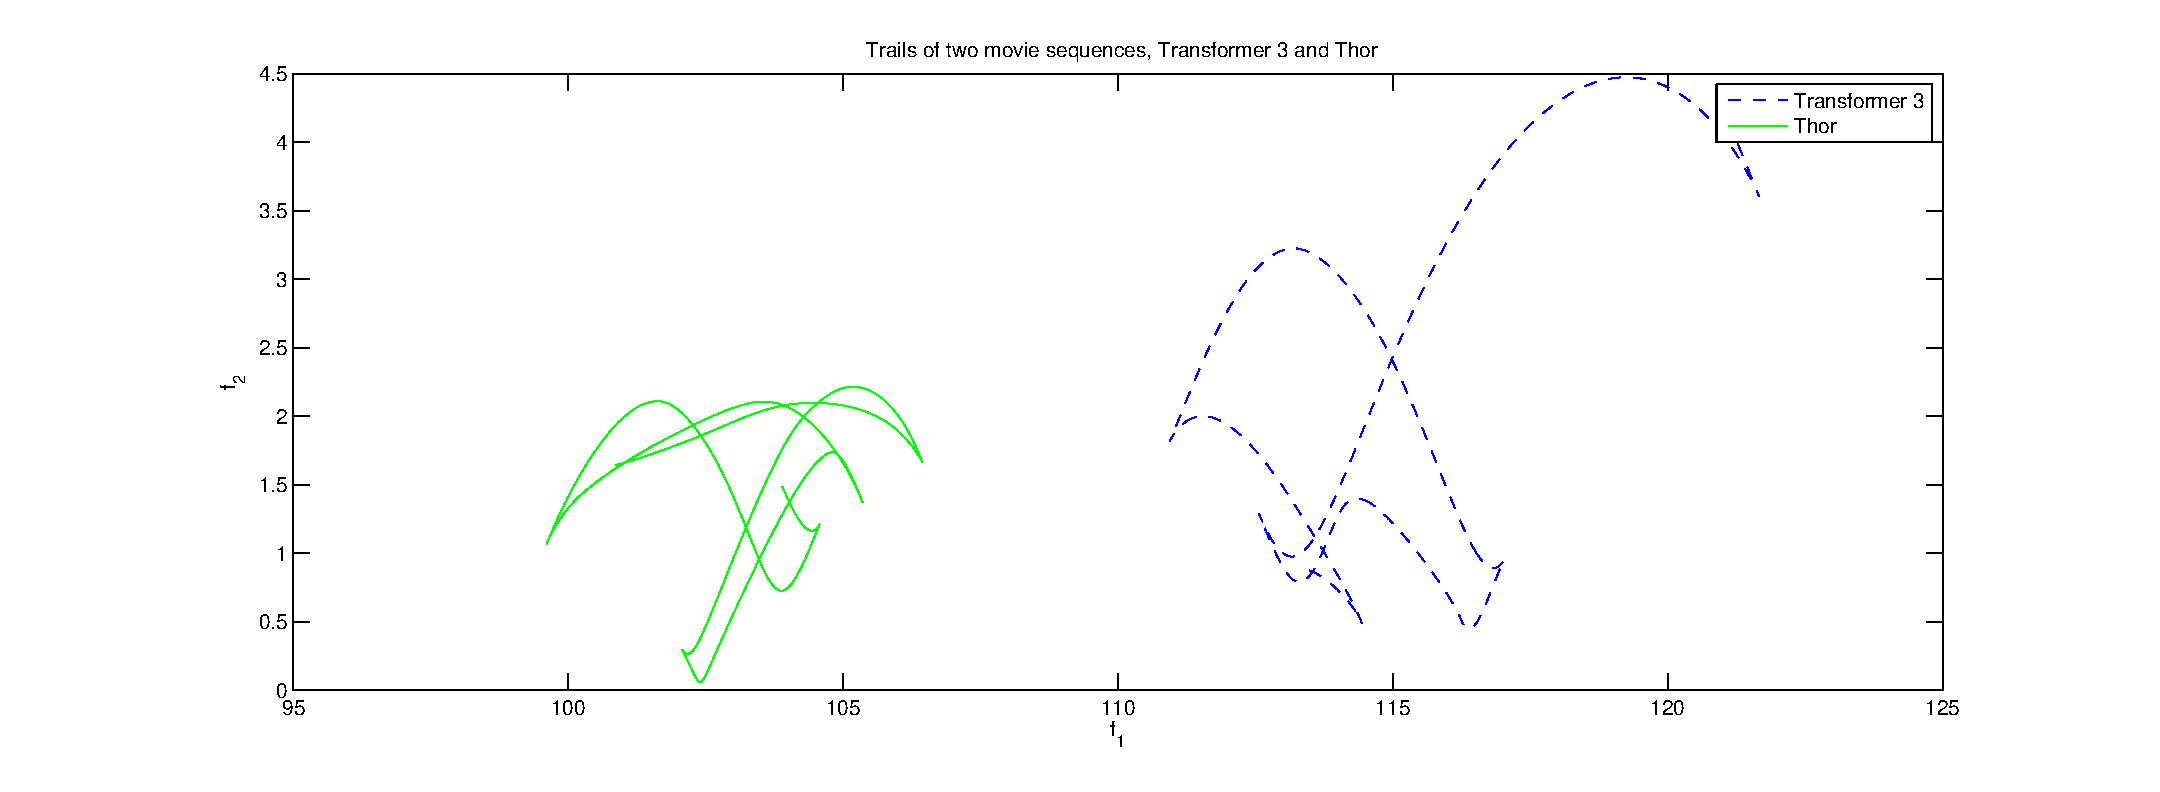
\includegraphics[scale=0.225]{Figures/MAP_TF_Thor}
	}
	\caption{(a)Two raw sequences, (b)two smoothed sequences, (c)five aligned sequences and averaged sequence and (d)a FFT filtered sequence}
\vspace{-5mm}
\end{figure}

\subsubsection{Storing processed sequence into a data structure:} 
For an efficient search operation, we decided to use R* tree\cite{Beckmann:1990}, which is a variant of R-tree. For first-approximation of spatial query, R* tree stores Minimum Bounding Rectangles (MBRs) that consist of multiple adjacent points in multi-dimensional space. In our project, the pre-processed video sequence can be depicted as a trail, which is a series of two-dimensional spatial points corresponding to the Fourier coefficients of each subsequence within the video sequence. On packing MBRs, the packing strategy used in \cite{Faloutsos:1994}\cite{Kamel:1993} is adopted to minimize the disk access cost in accessing a specific node in R* tree.